\documentclass[12pt,a4paper]{article}
\usepackage{algorithm, algpseudocode, amsmath, amssymb, amsthm, csquotes, empheq, geometry, graphicx, hyperref, listings, multirow, siunitx, subcaption, upgreek}
\usepackage[italicdiff]{physics}
\usepackage[section]{placeins}
\usepackage[justification=centering]{caption}

\title{Computational Physics\\Problem Set 8}
\author{Saleh Shamloo Ahmadi\\Student Number: 98100872}
\date{Decebmer 6, 2021}

\hypersetup{colorlinks=true, urlcolor=cyan}
\newcommand{\fig}{../fig}
\newcommand{\ddfrac}[2]{{\displaystyle\frac{\displaystyle #1}{\displaystyle #2}}}
\newcommand{\multlinecell}[1]{\begin{tabular}[c]{@{}c@{}}#1\end{tabular}}

\begin{document}
	\maketitle
	In this problem set we simulate the 2D Ising model in a rectangular lattice with no external magnetic field
	and periodic boundary conditions using the Metropolis Monte Carlo method.
	\begin{equation}
		E = -J\sum_i\sum_{j\in\text{neighbors($i$)}}\sigma_i\sigma_j;\qquad
		\sigma=\left\{\begin{gathered}
			+1\\-1
		\end{gathered}\right.
	\end{equation}

	To speed up the algorithm, the spins can be updated in a checkerboard pattern with vectorized
	caclulations\footnote{Source: Joshua, R.; Mauro, B.; Massimiliano, F.; Massimo, B.;
	\textit{A Performance Study of the 2D Ising Model on GPUs} \href{https://arxiv.org/abs/1906.06297}{arXiv.org link}},
	as demonstrated in figure \ref{fig:checkerboard}.

	Notes:
	\begin{enumerate}
		\item Relaxation time varies with the temperature and the size of the lattice, but it is generally small
		compared to my simulation times. I took the relaxation time to be a tenth of the simulation time. 
		\item In small lattices, the correlation length is hard to measure and diverges easily, so the data for lattice
		sidelengths 8 and 16 is omitted.
		\item Due to the \enquote{freezing} effect, outliers are common in low temperatures and ruin the data. For large
		sidelengths, an enormous amount of data is needed to correct the effect of the outliers. Because of this,
		I smoothed out the curves for the sidelengths 256 and 512 by hand.
	\end{enumerate}

	Also, I made some \texttt{gif}s which can be found under the \texttt{anim} directory.
	\begin{figure}
		\centering
		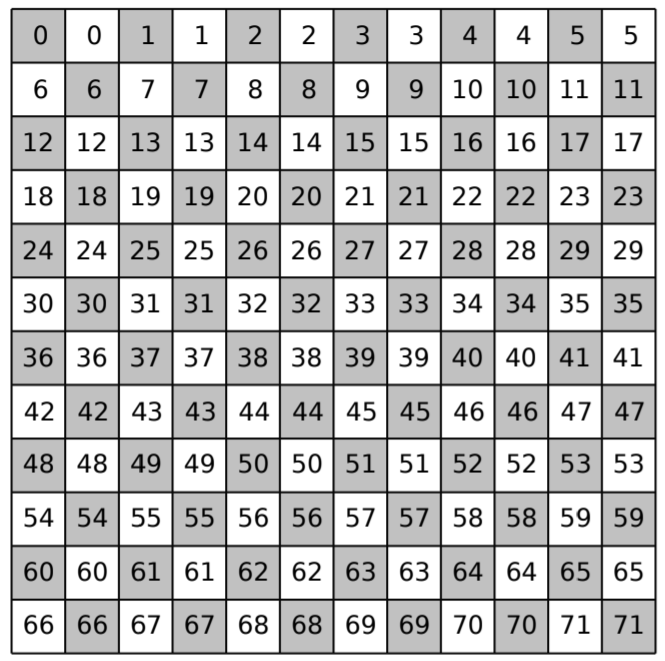
\includegraphics[width=0.8\linewidth]{checkerboard.png}
		\caption{the cells of each \enquote{color} do not interact with each other, so they can be updated all
			at the same time}
		\label{fig:checkerboard}
	\end{figure}
	\begin{table}
		\centering
		\caption{For calculating $\xi$, only sidelengths 32, 64, 128, and 256 were used. For calculating $\chi$
			sidelength 512 was not used due to low accuracy. The actual values (coming directly from theory)
			for $\nu$, $\gamma$, and $\beta$ are 1, $7/4=1.75$, and $1/8=0.125$. So as you can see, the calculated
			values are fairly close to the actual theoretical values.}
		\begin{tabular}{|c|c|c|c|}
			\hline
			Relation & \multicolumn{2}{|c|}{Critical Exponent} & $T_c(\infty)$ \\
			\hline
			$\xi\sim L\sim \abs{T_c-T}^{-\nu}$ & $\nu$ & 0.91 & 2.264 \\
			$C_V\sim c_0\ln{\abs{T_c-T}}$ & $c_0$ & -0.56 & 2.265 \\
			$\chi\sim\abs{T_c-T}^{-\gamma}$ & $\gamma$ & 1.70 & 2.264 \\
			$\expval{\abs{m}}\sim\abs{T_c-T}^{\beta}$ & $\beta$ & 0.123 & 2.270 \\
			\hline
		\end{tabular}
	\end{table}

	\newgeometry{top=0.5in, bottom=1in, left=0.5in, right=0.5in}
	\begin{figure}[htb!]
		\centering
		\begin{subfigure}{0.45\linewidth}
			\centering
			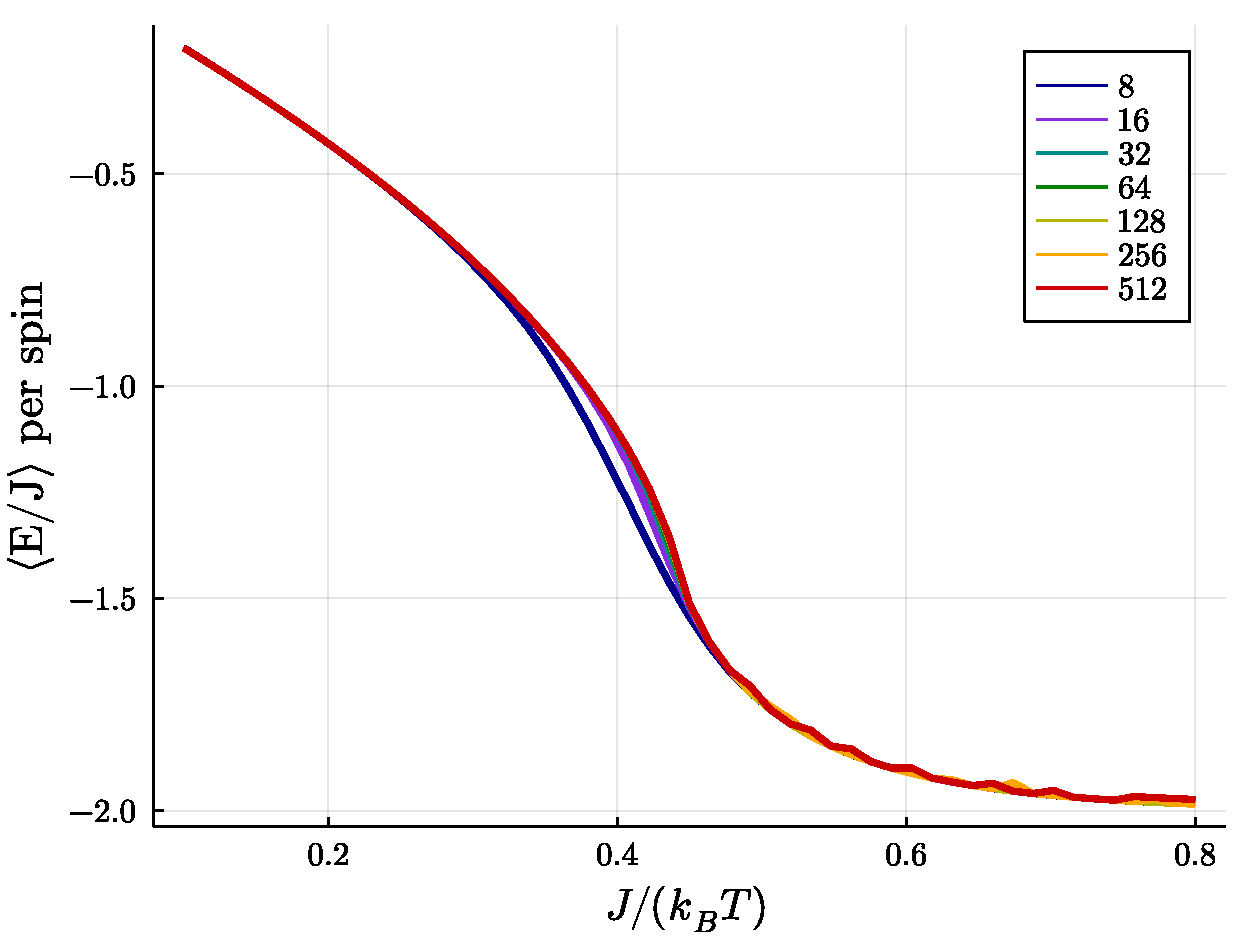
\includegraphics[width=\linewidth]{\fig/energy-full}
		\end{subfigure}
		\begin{subfigure}{0.45\linewidth}
			\centering
			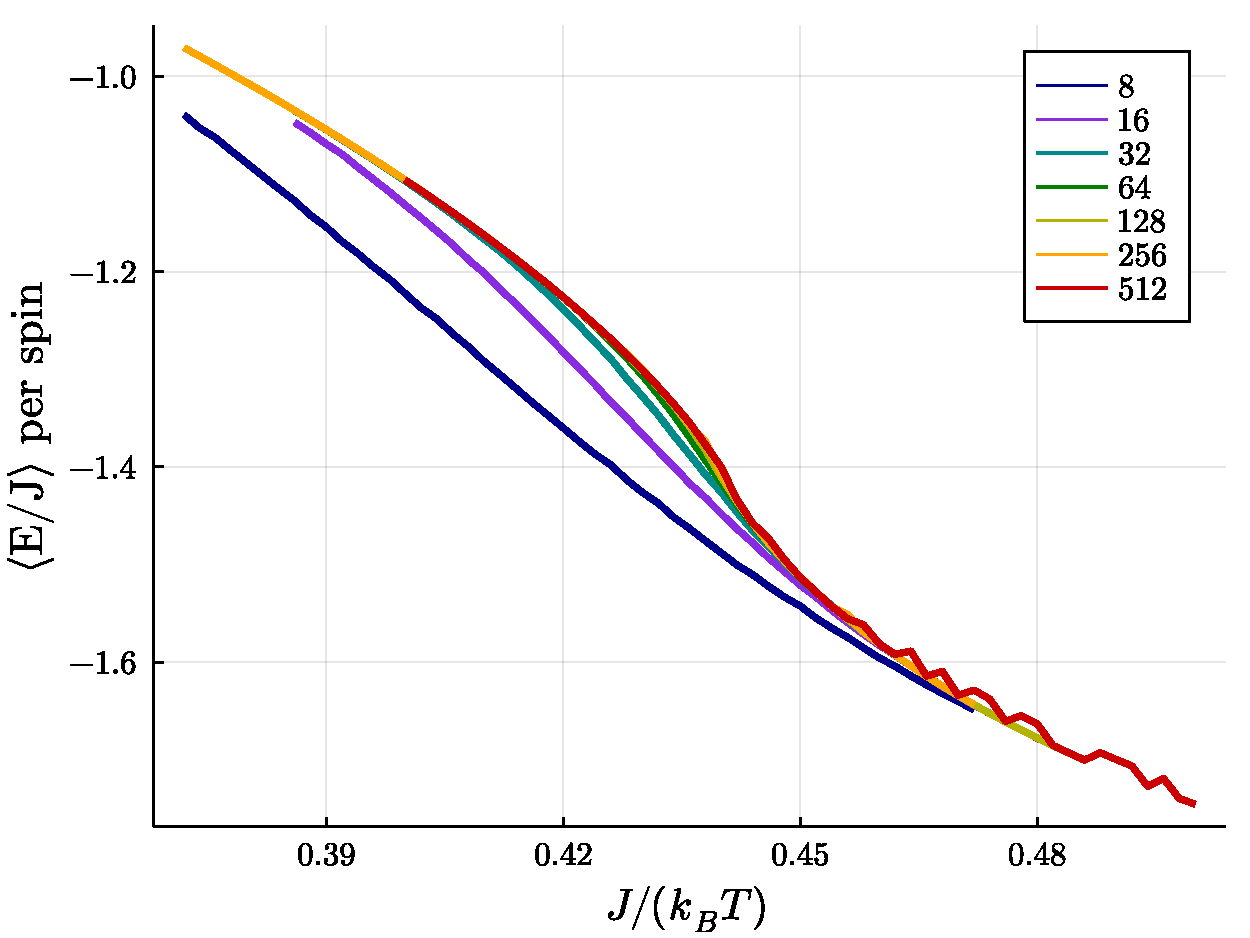
\includegraphics[width=\linewidth]{\fig/energy-zoom}
		\end{subfigure}
		\caption{Energy}
	\end{figure}
	\begin{figure}[htb!]
		\centering
		\begin{subfigure}{0.45\linewidth}
			\centering
			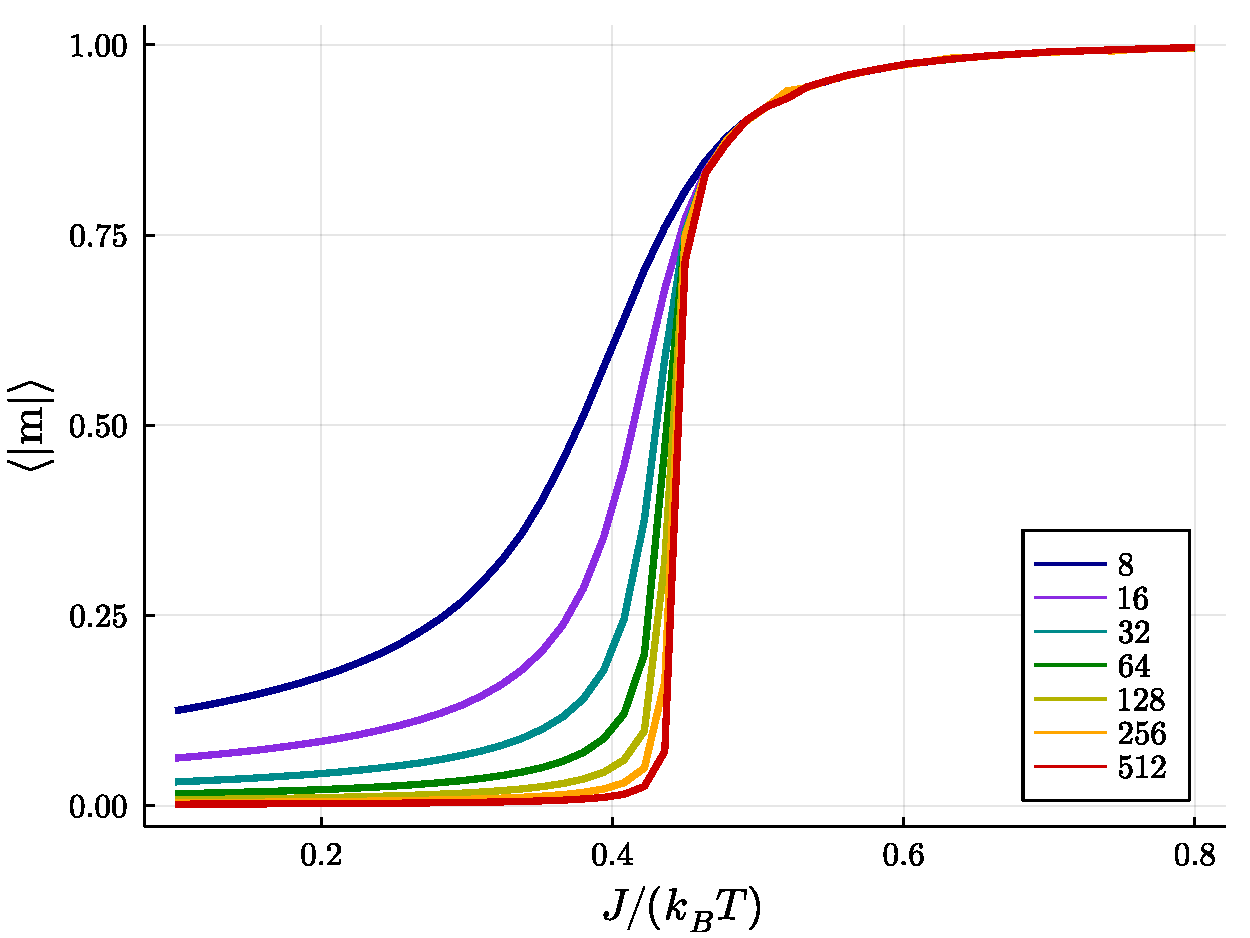
\includegraphics[width=\linewidth]{\fig/magnetization-full}
		\end{subfigure}
		\begin{subfigure}{0.45\linewidth}
			\centering
			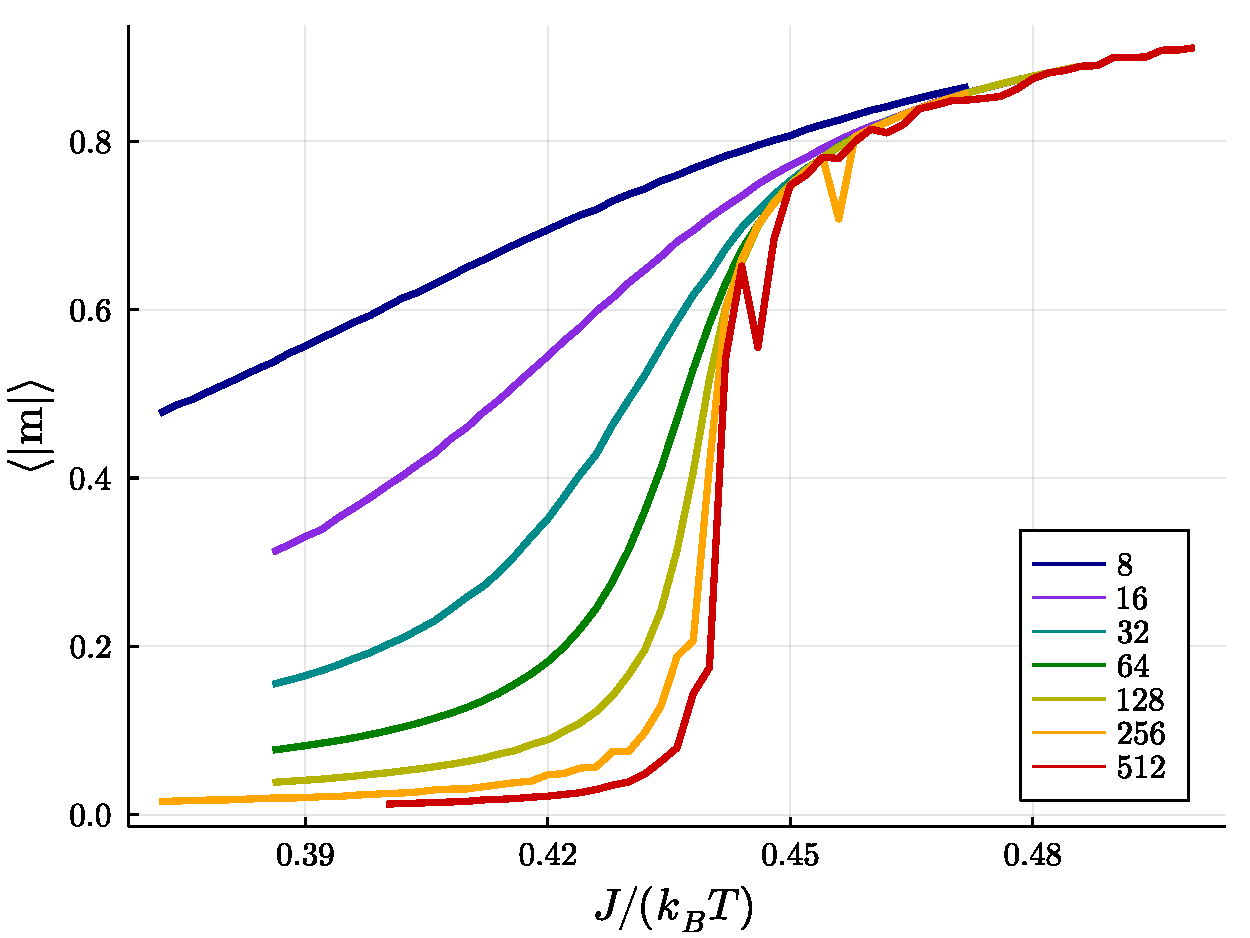
\includegraphics[width=\linewidth]{\fig/magnetization-zoom}
		\end{subfigure}
		\caption{Magnetization (mean spin)}
	\end{figure}
	\begin{figure}[htb!]
		\centering
		\begin{subfigure}{0.45\linewidth}
			\centering
			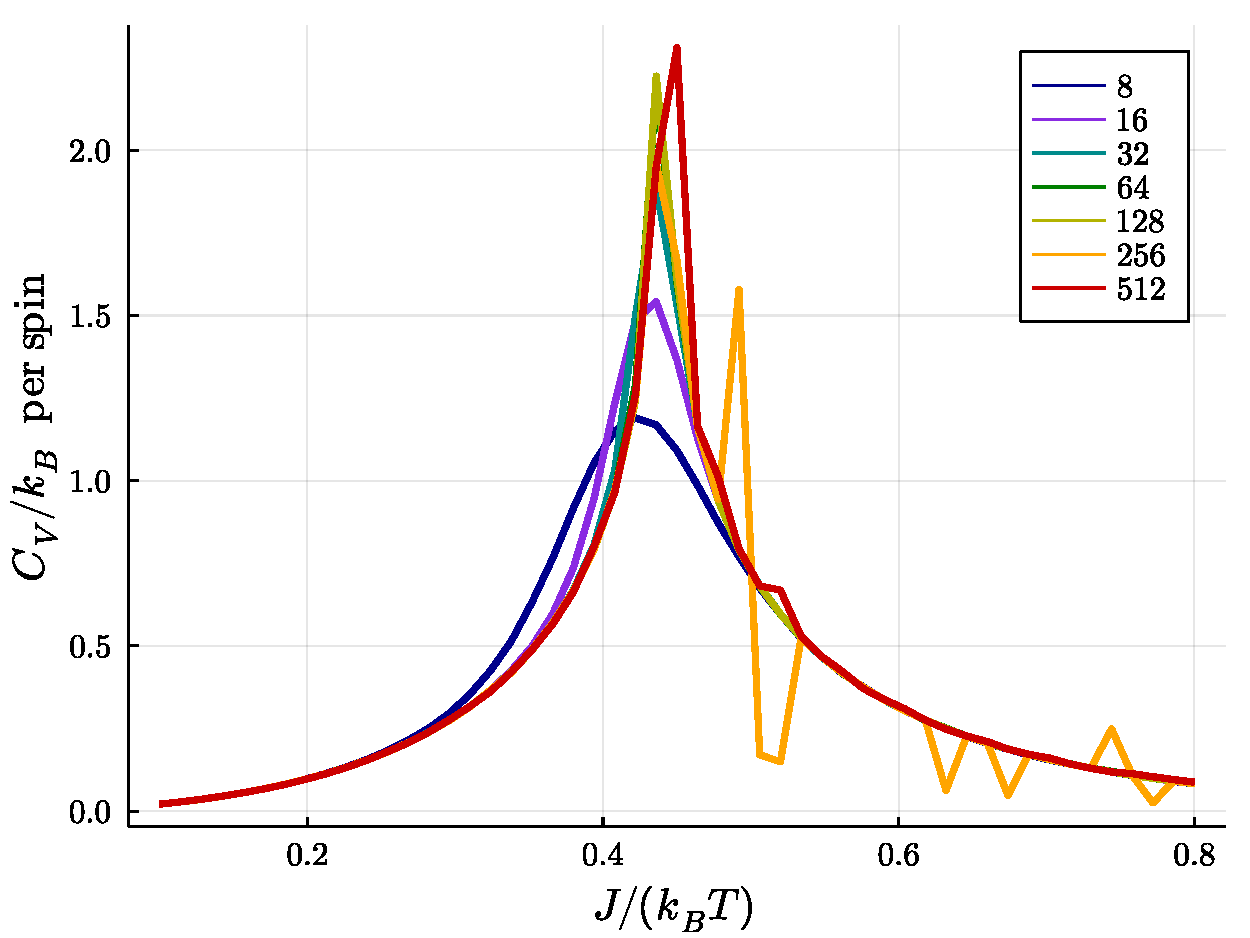
\includegraphics[width=\linewidth]{\fig/Cv-full}
		\end{subfigure}
		\begin{subfigure}{0.45\linewidth}
			\centering
			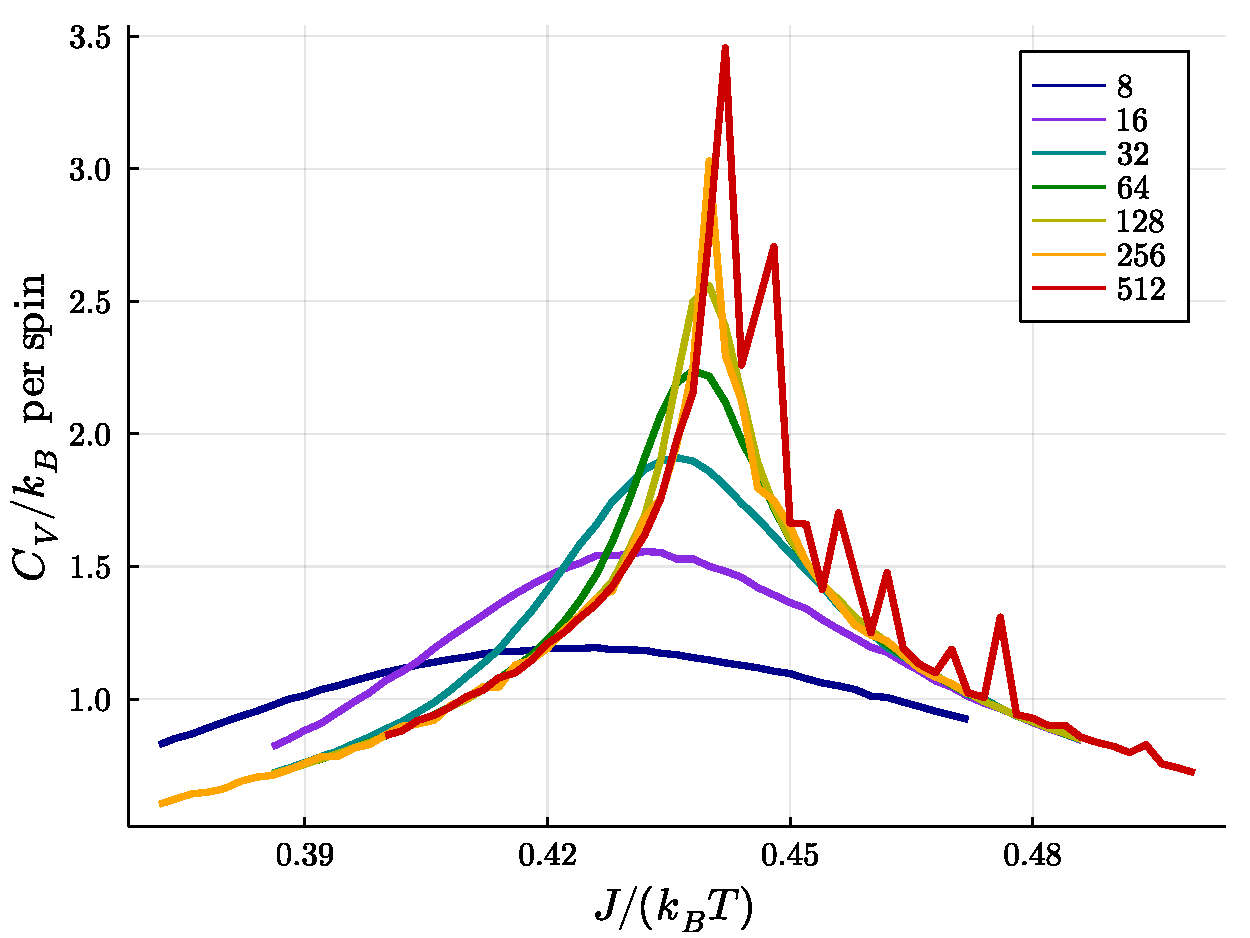
\includegraphics[width=\linewidth]{\fig/Cv-zoom}
		\end{subfigure}
		\caption{Heat Capacity $C_V$}
	\end{figure}
	\begin{figure}[htb!]
		\centering
		\begin{subfigure}{0.45\linewidth}
			\centering
			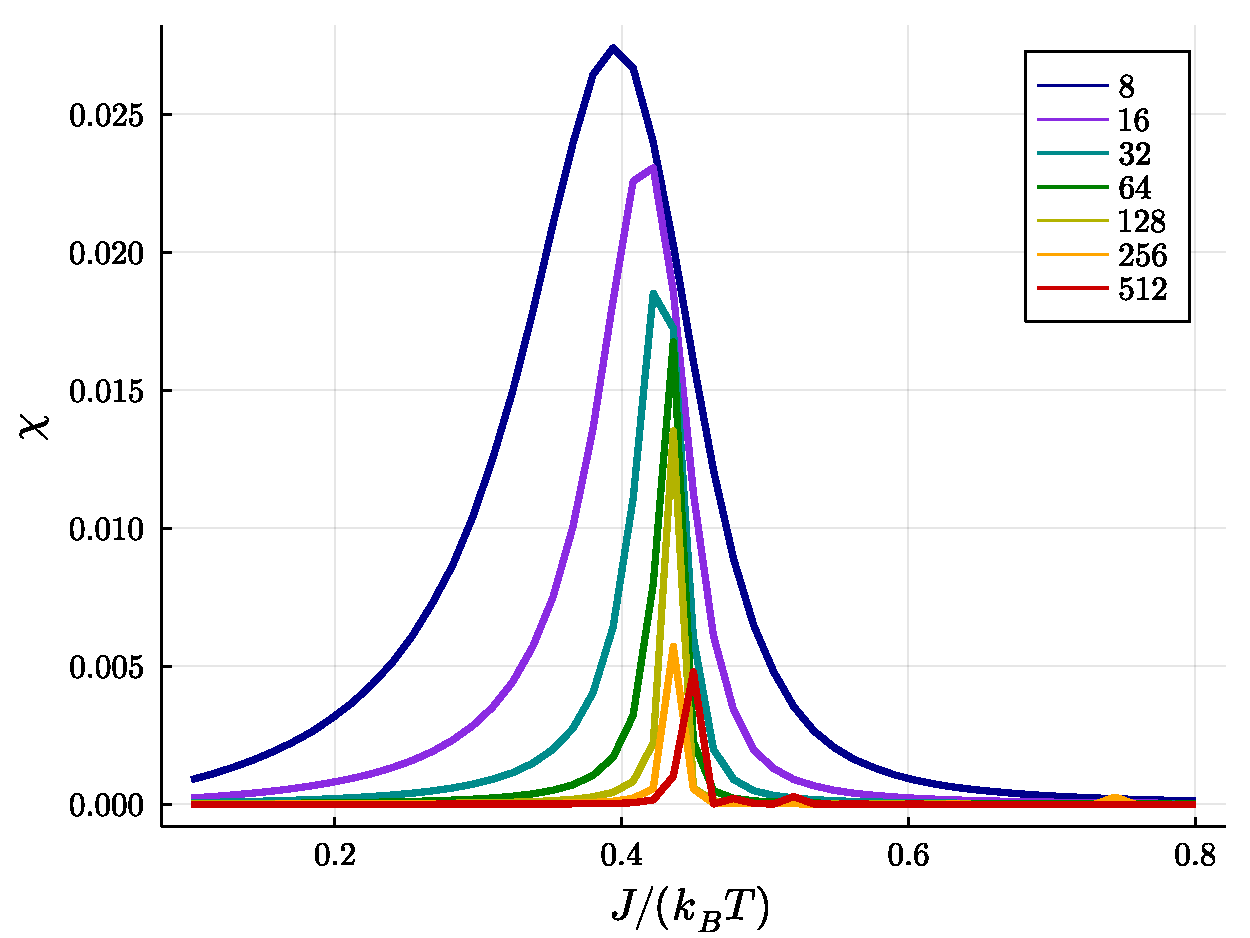
\includegraphics[width=\linewidth]{\fig/chi-full}
		\end{subfigure}
		\begin{subfigure}{0.45\linewidth}
			\centering
			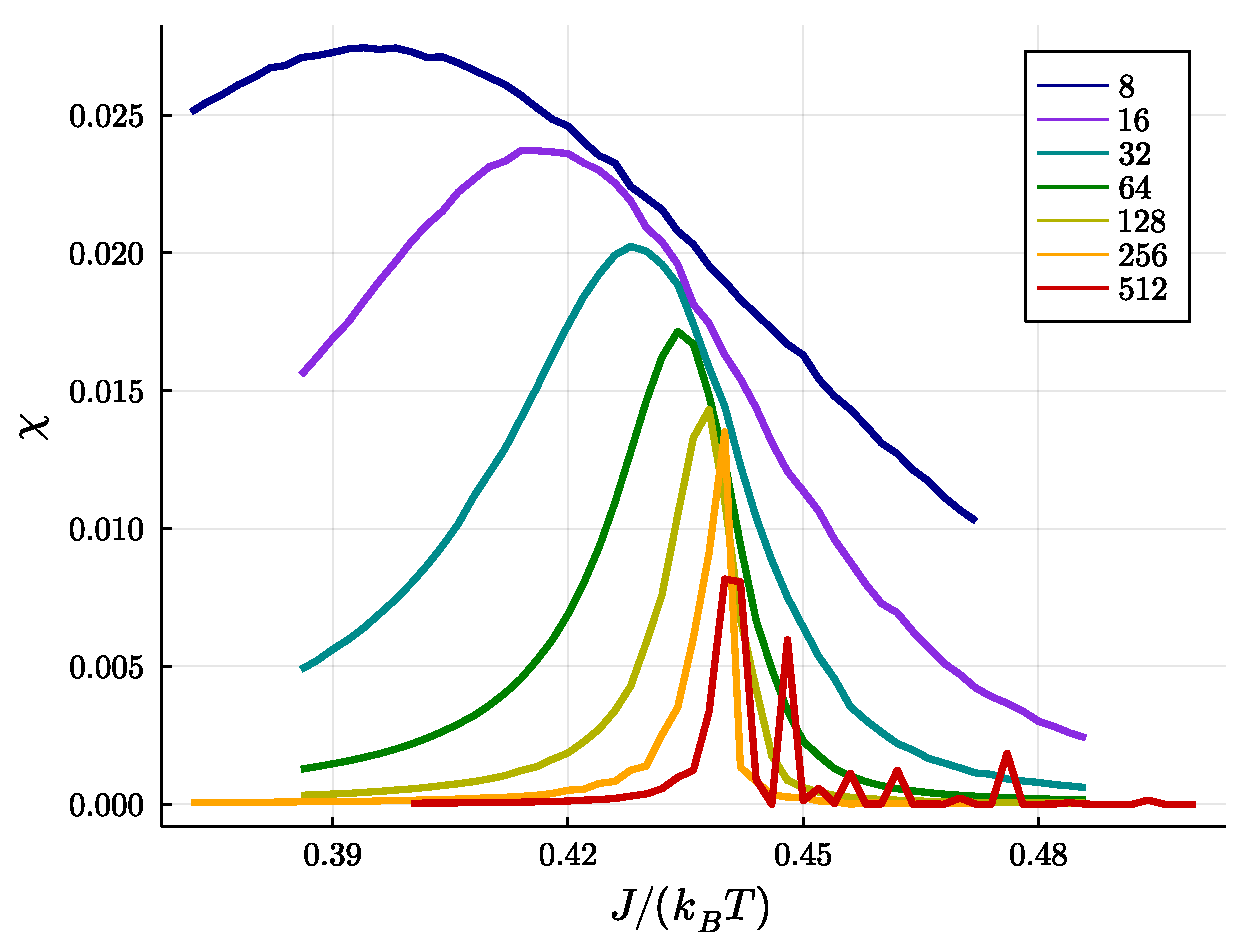
\includegraphics[width=\linewidth]{\fig/chi-zoom}
		\end{subfigure}
		\caption{Magnetic Susceptibility $\chi$}
	\end{figure}
	\begin{figure}[htb!]
		\centering
		\begin{subfigure}{0.45\linewidth}
			\centering
			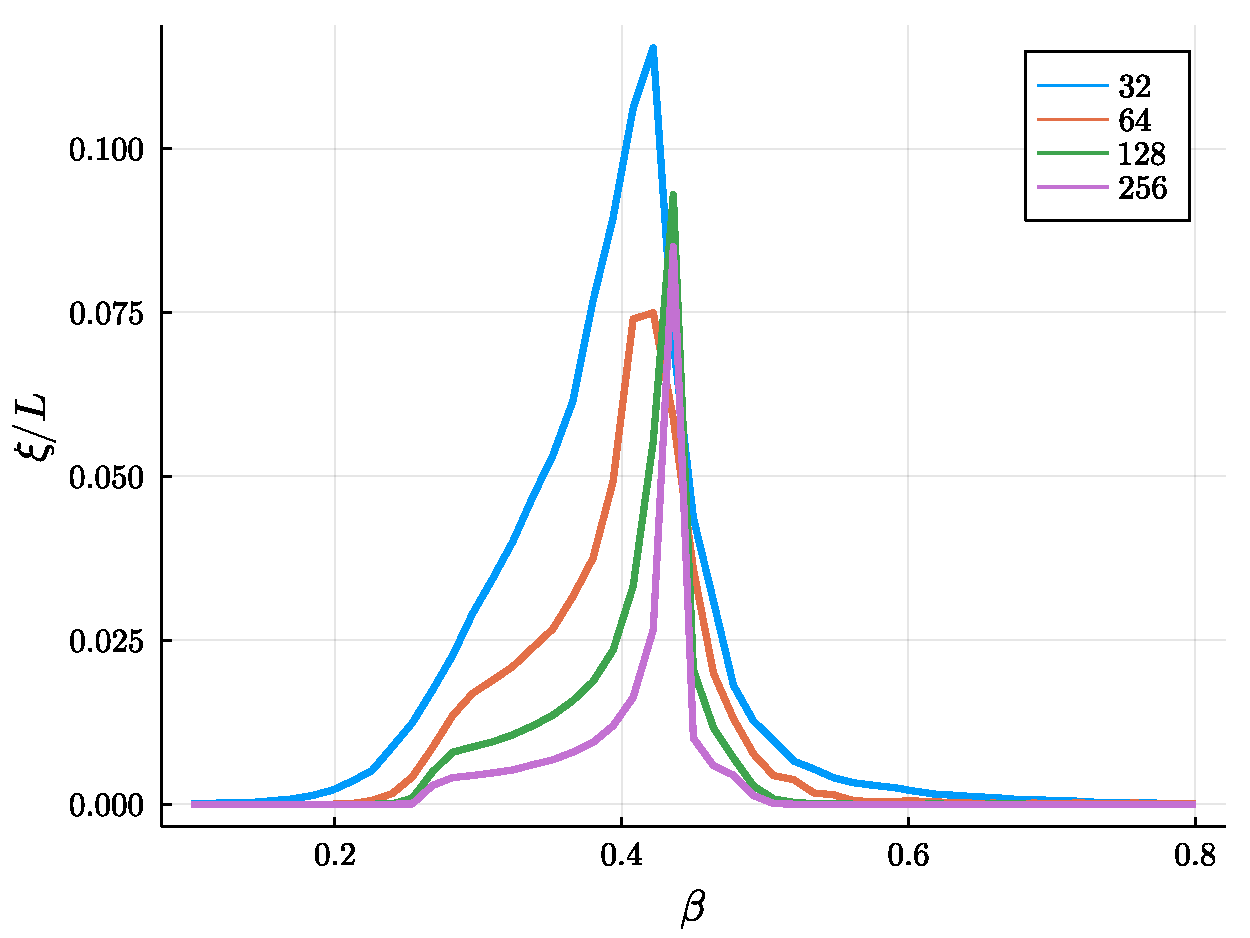
\includegraphics[width=\linewidth]{\fig/xi-full}
		\end{subfigure}
		\begin{subfigure}{0.45\linewidth}
			\centering
			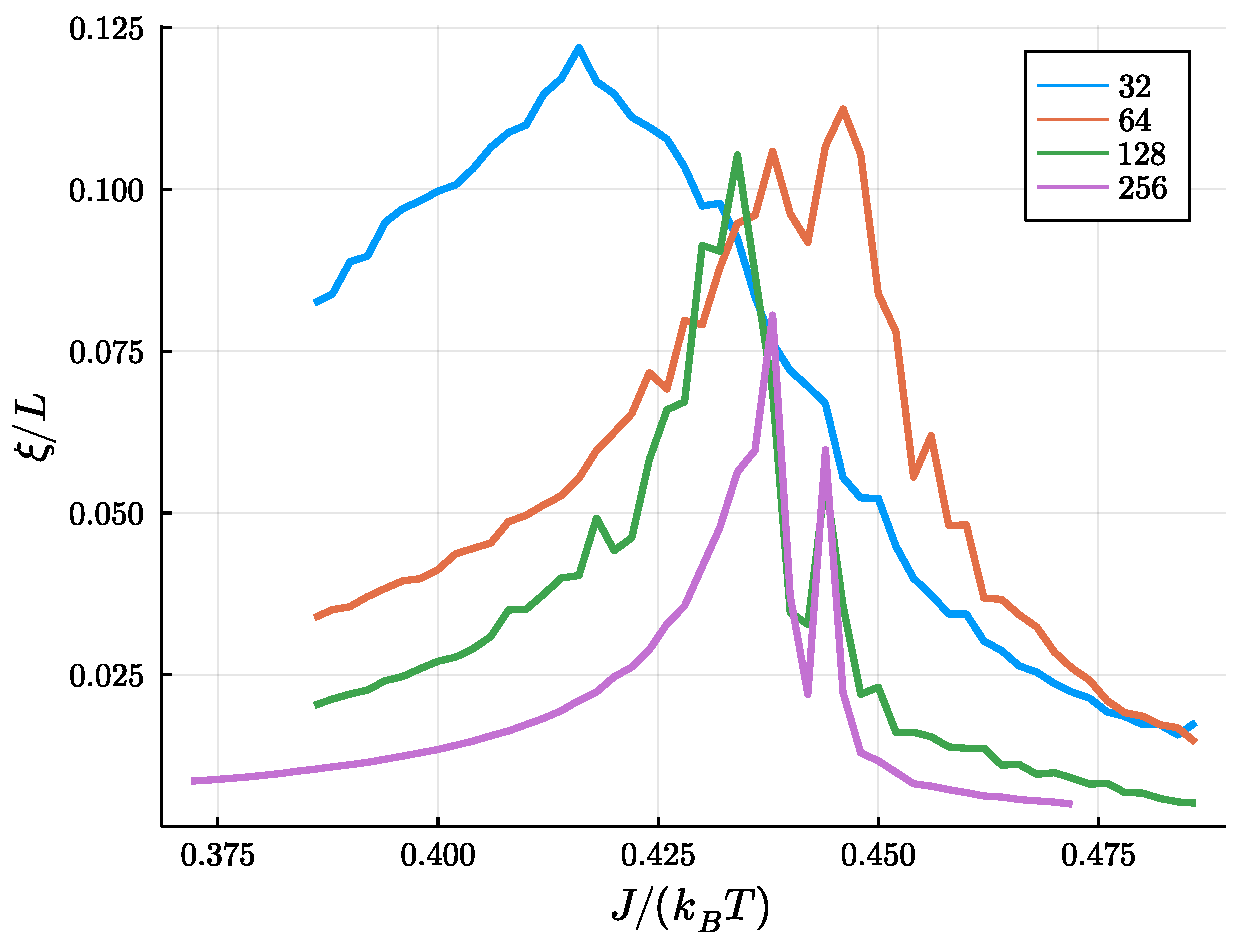
\includegraphics[width=\linewidth]{\fig/xi-zoom}
		\end{subfigure}
		\caption{Correlation Length $\xi$}
	\end{figure}

	\begin{figure}[htb!]
		\centering
		\begin{subfigure}{0.45\linewidth}
			\centering
			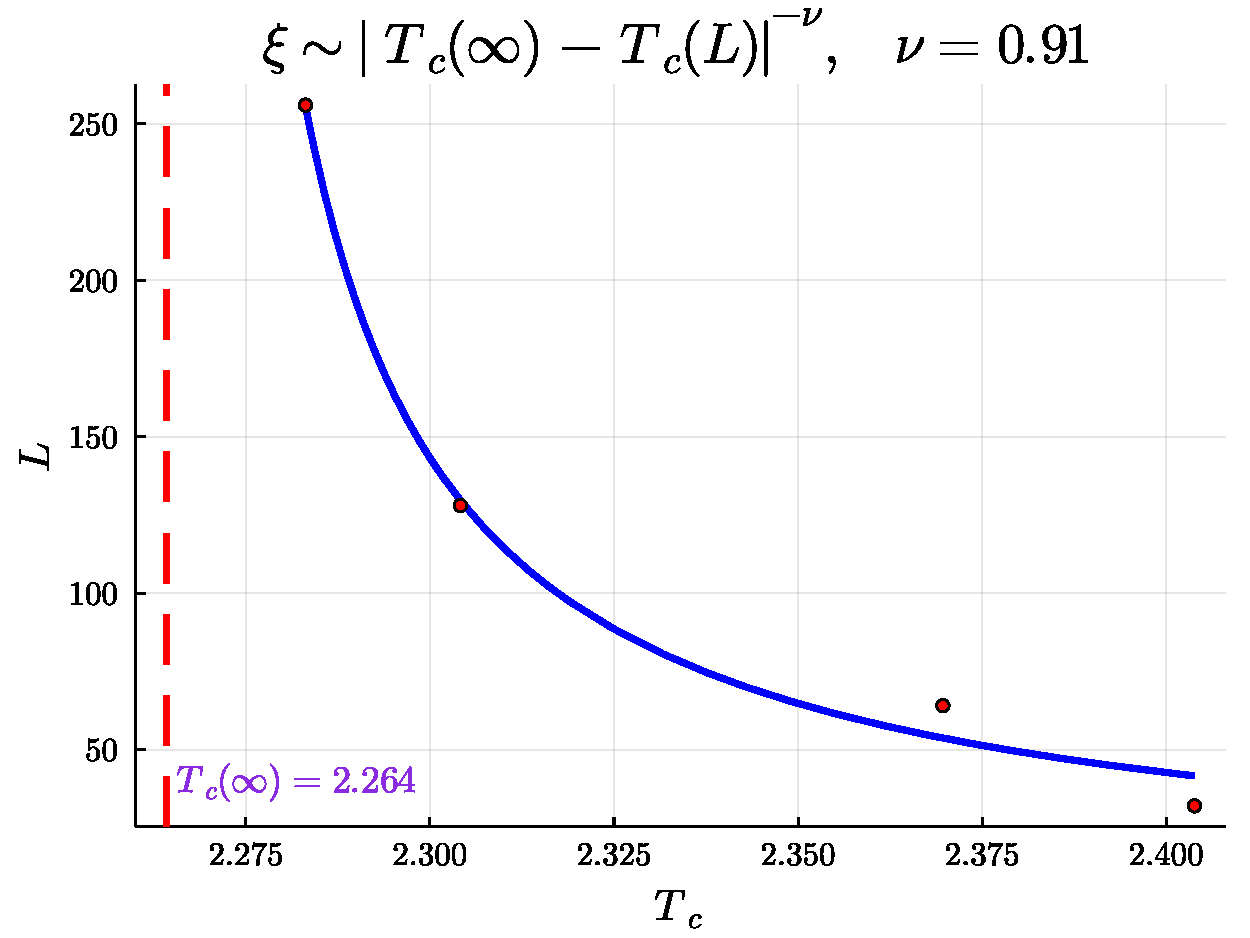
\includegraphics[width=\linewidth]{\fig/fit-xi}
		\end{subfigure}
		\begin{subfigure}{0.45\linewidth}
			\centering
			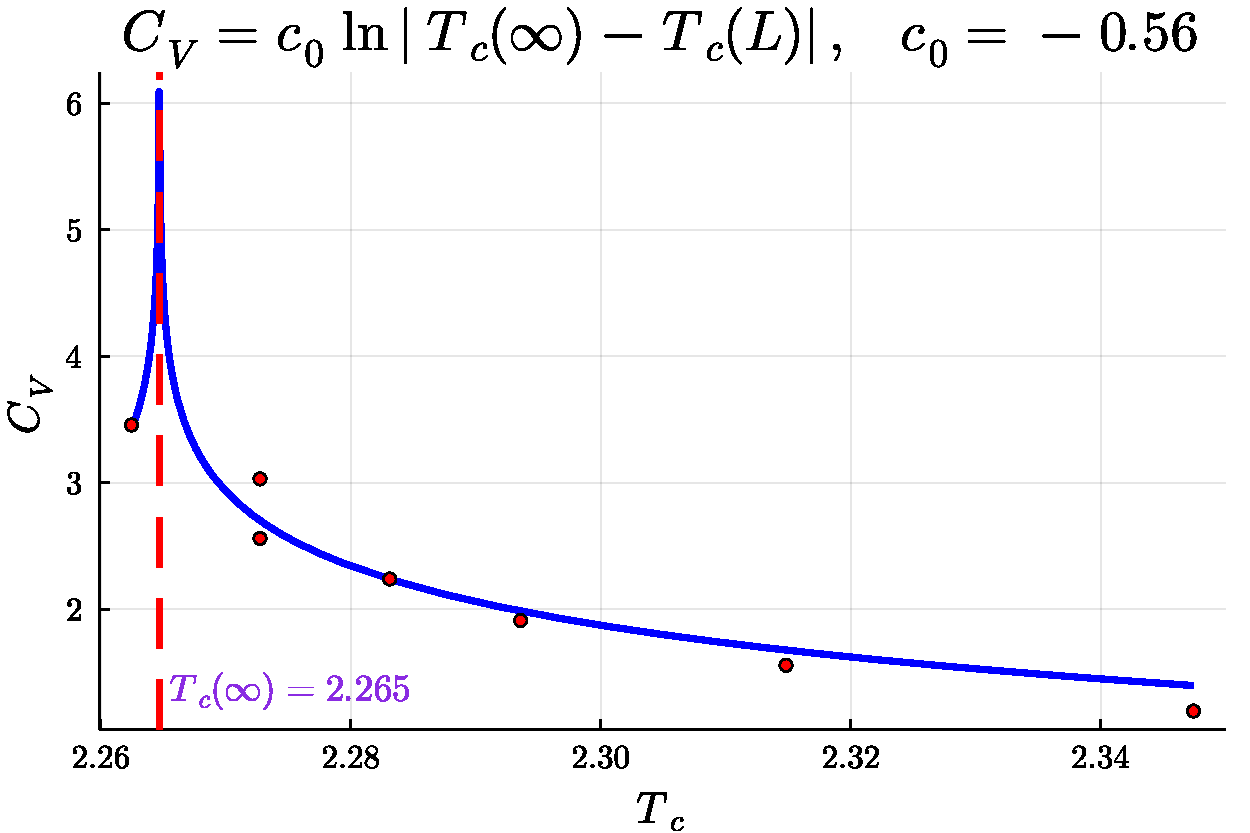
\includegraphics[width=\linewidth]{\fig/fit-Cv}
		\end{subfigure}
	\end{figure}
	\begin{figure}[htb!]
		\centering
		\begin{subfigure}{0.45\linewidth}
			\centering
			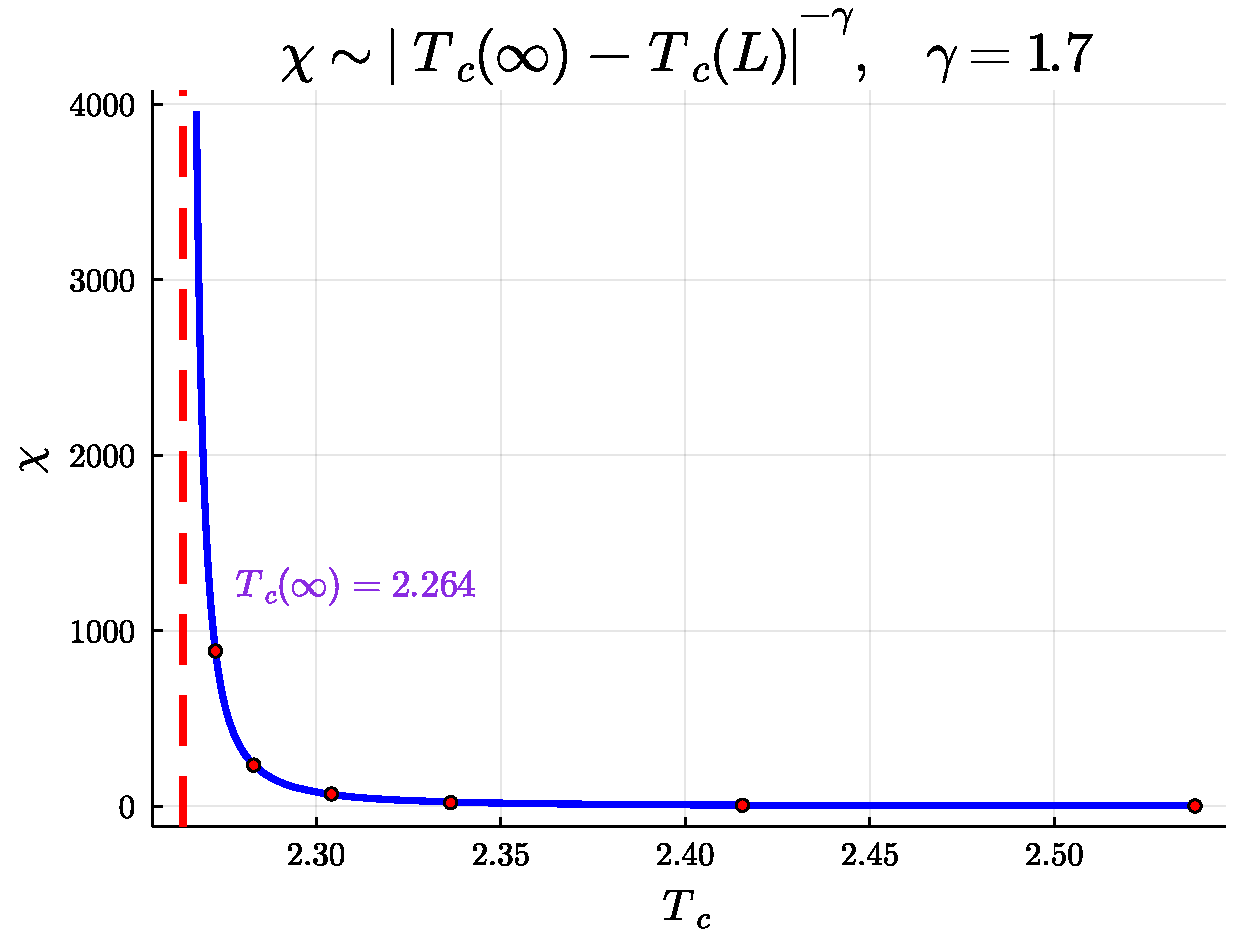
\includegraphics[width=\linewidth]{\fig/fit-chi}
		\end{subfigure}
		\begin{subfigure}{0.45\linewidth}
			\centering
			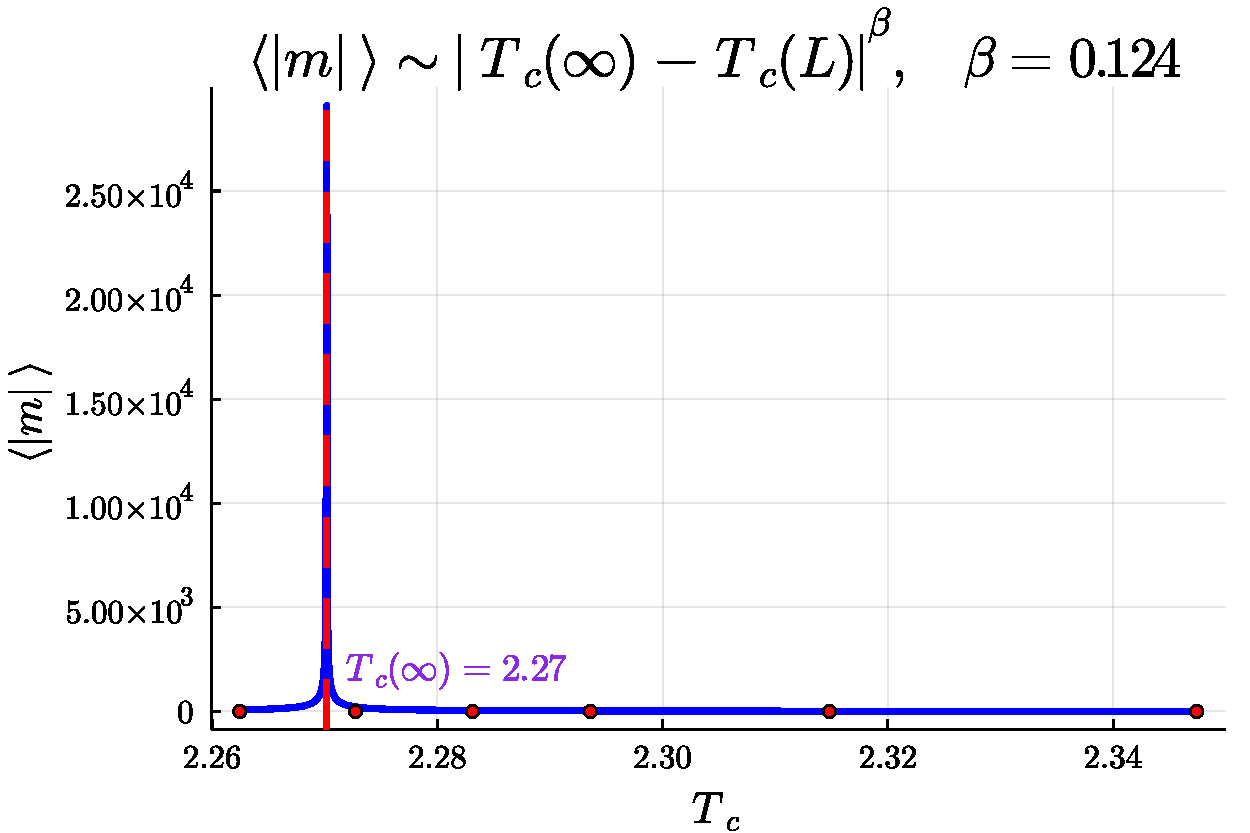
\includegraphics[width=\linewidth]{\fig/fit-magnetization}
		\end{subfigure}
	\end{figure}

	\begin{figure}[htb!]
		\centering
		\begin{subfigure}{0.4\linewidth}
			\centering
			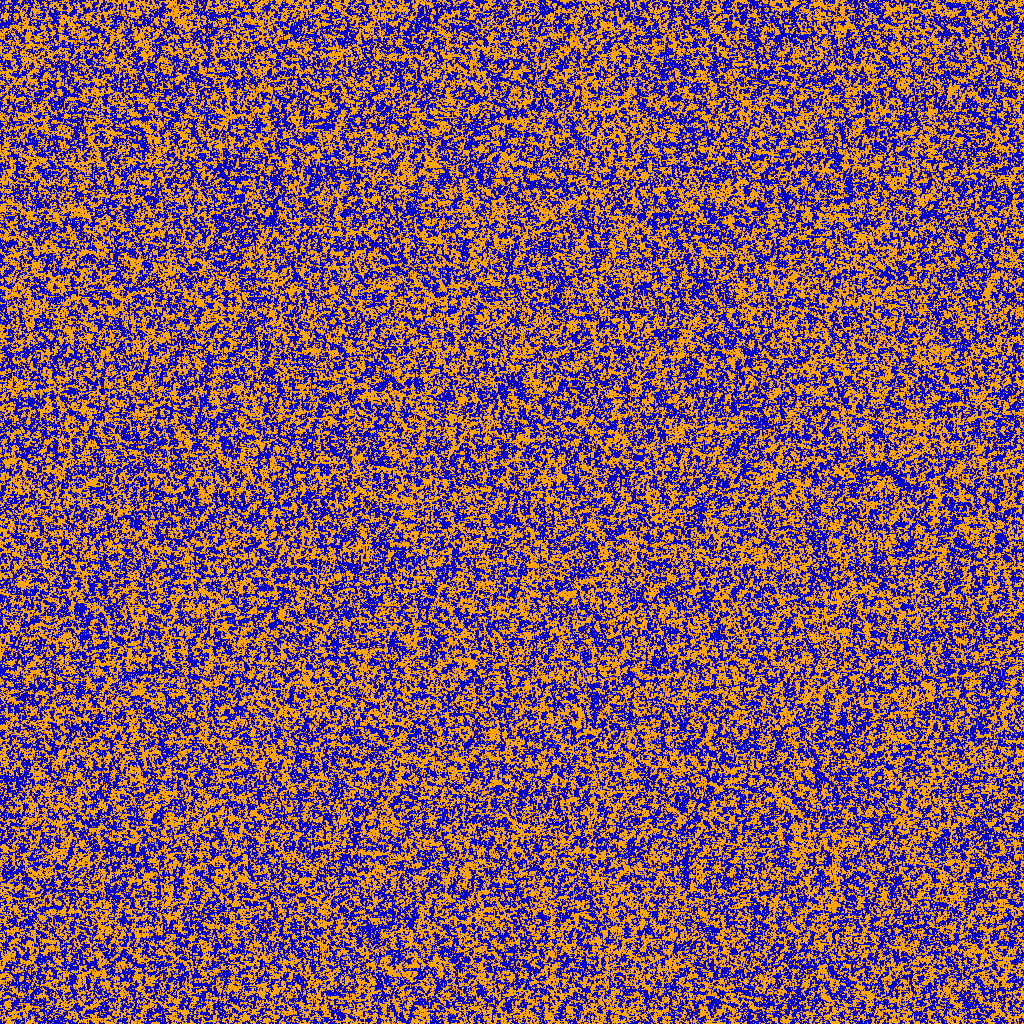
\includegraphics[width=\linewidth]{\fig/vis-0.3}
			\caption*{$J/(k_B T) = 0.3$}
		\end{subfigure}
		\begin{subfigure}{0.4\linewidth}
			\centering
			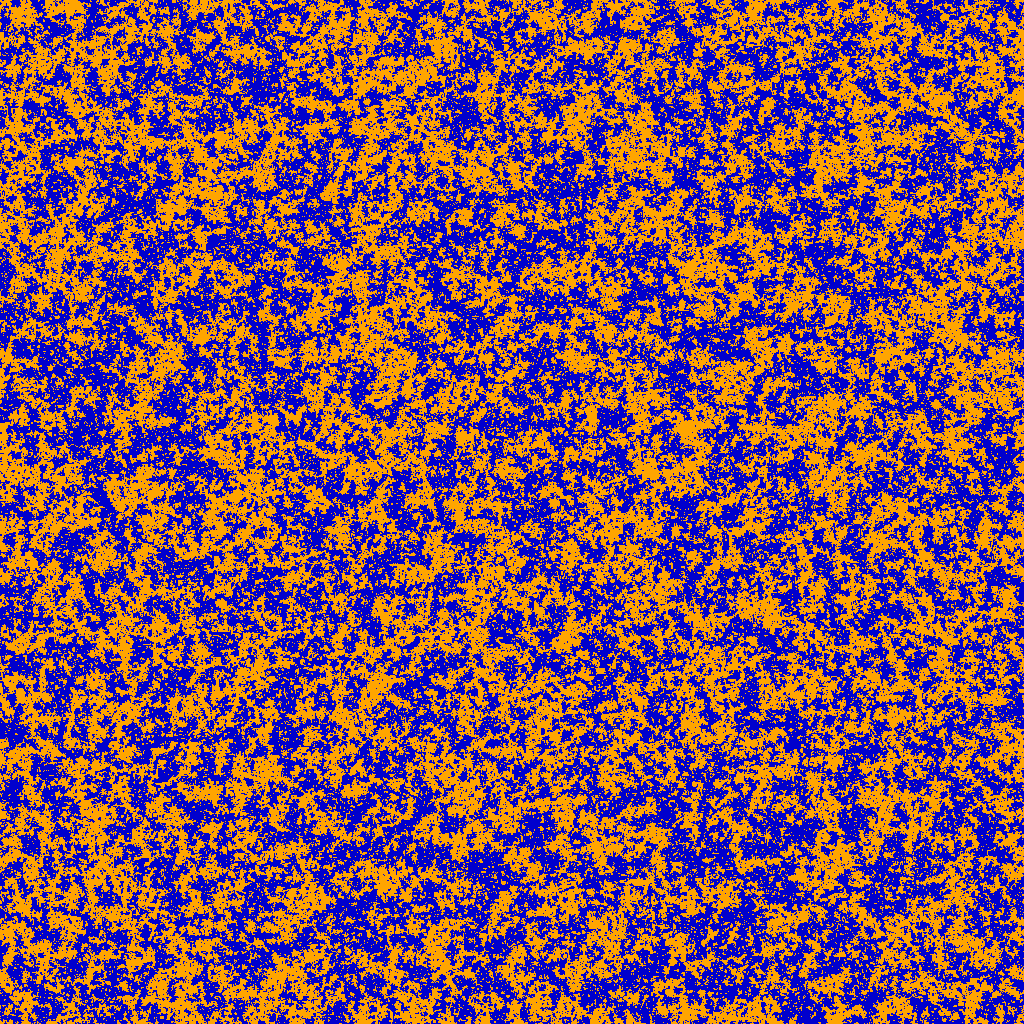
\includegraphics[width=\linewidth]{\fig/vis-0.4}
			\caption*{$J/(k_B T) = 0.4$}
		\end{subfigure}
		\begin{subfigure}{0.4\linewidth}
			\centering
			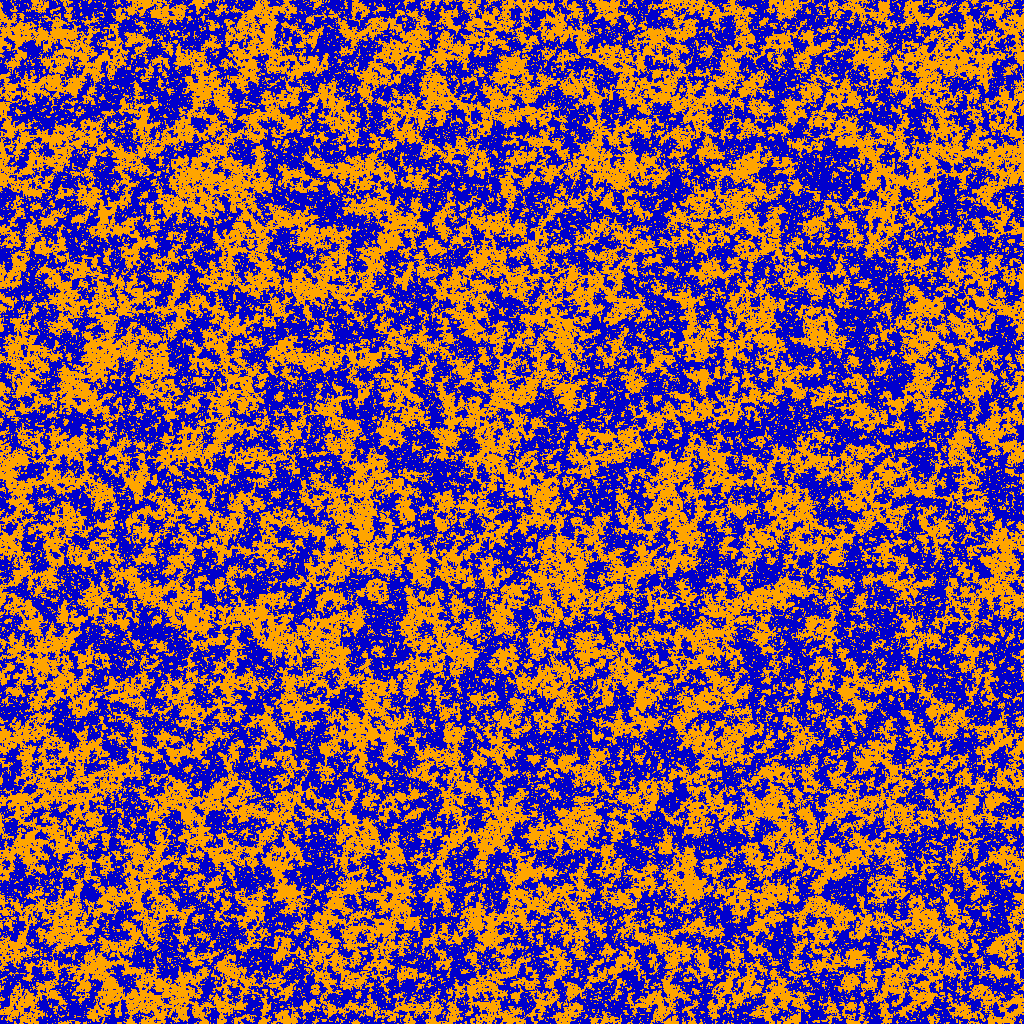
\includegraphics[width=\linewidth]{\fig/vis-0.41}
			\caption*{$J/(k_B T) = 0.41$}
		\end{subfigure}
		\begin{subfigure}{0.4\linewidth}
			\centering
			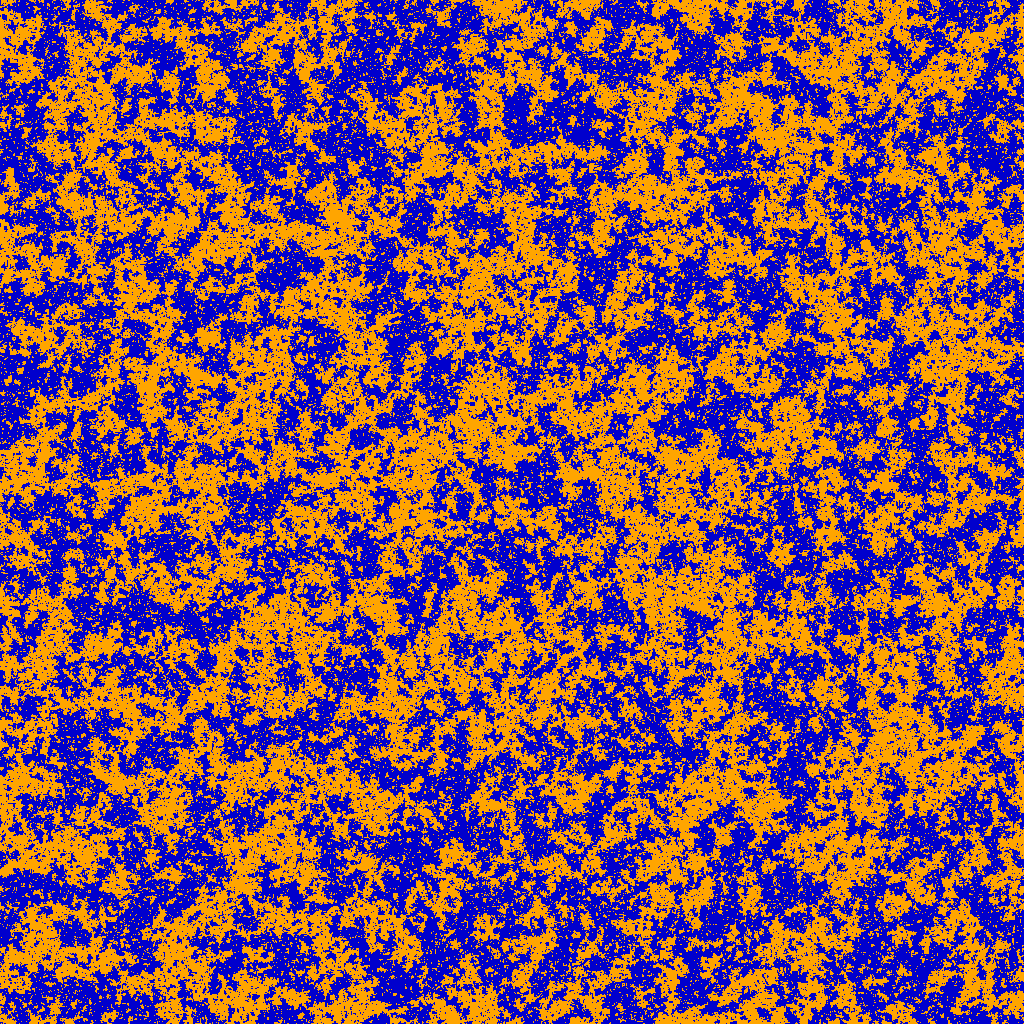
\includegraphics[width=\linewidth]{\fig/vis-0.42}
			\caption*{$J/(k_B T) = 0.42$}
		\end{subfigure}
	\end{figure}
	\begin{figure}[htb!]
		\centering
		\begin{subfigure}{0.4\linewidth}
			\centering
			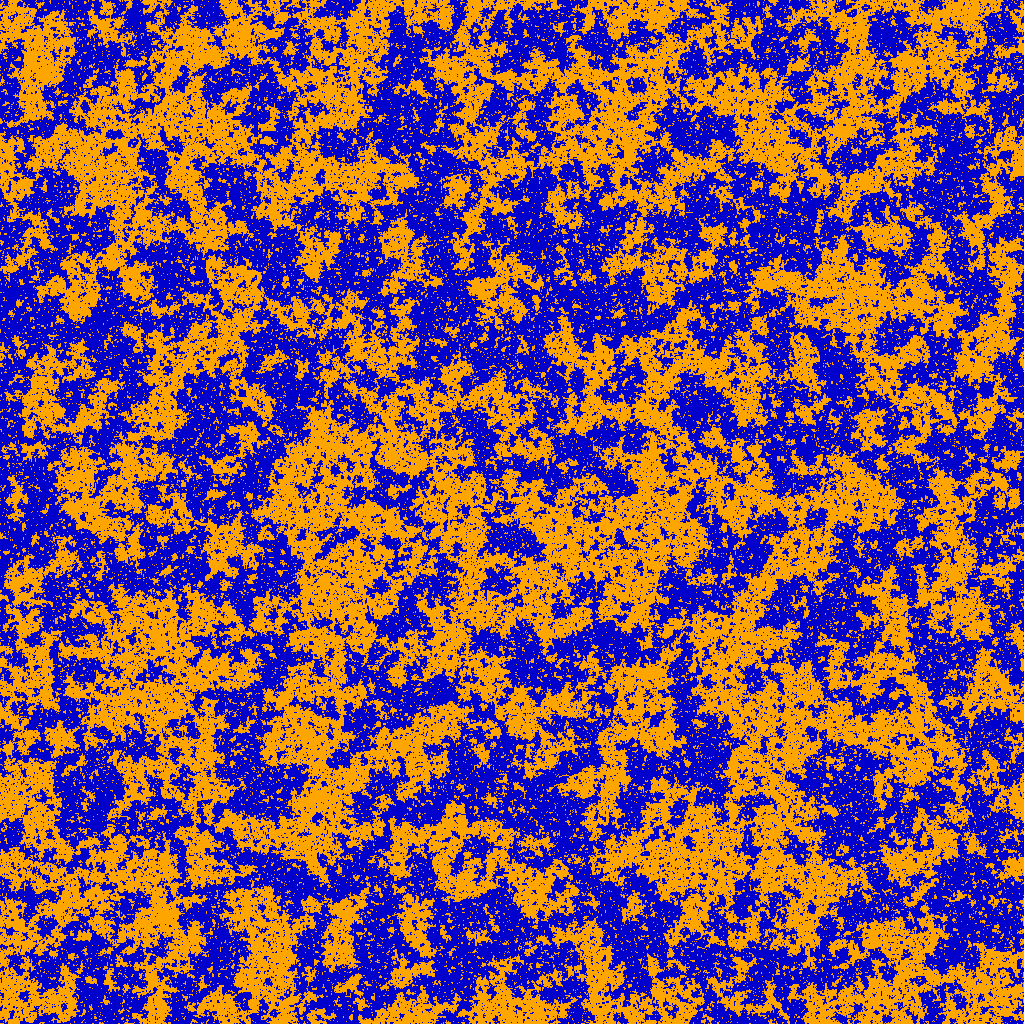
\includegraphics[width=\linewidth]{\fig/vis-0.43}
			\caption*{$J/(k_B T) = 0.43$}
		\end{subfigure}
		\begin{subfigure}{0.4\linewidth}
			\centering
			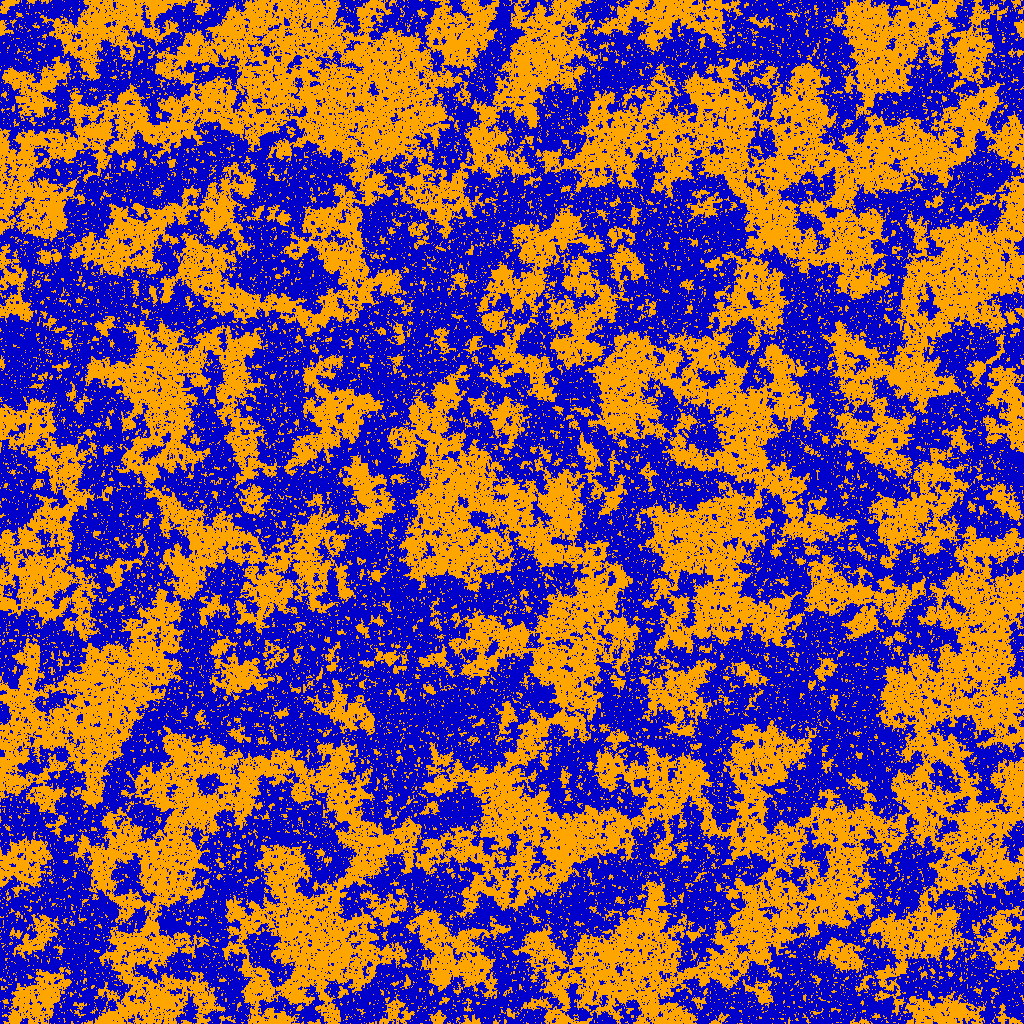
\includegraphics[width=\linewidth]{\fig/vis-0.44}
			\caption*{$J/(k_B T) = 0.44$}
		\end{subfigure}
		\begin{subfigure}{0.4\linewidth}
			\centering
			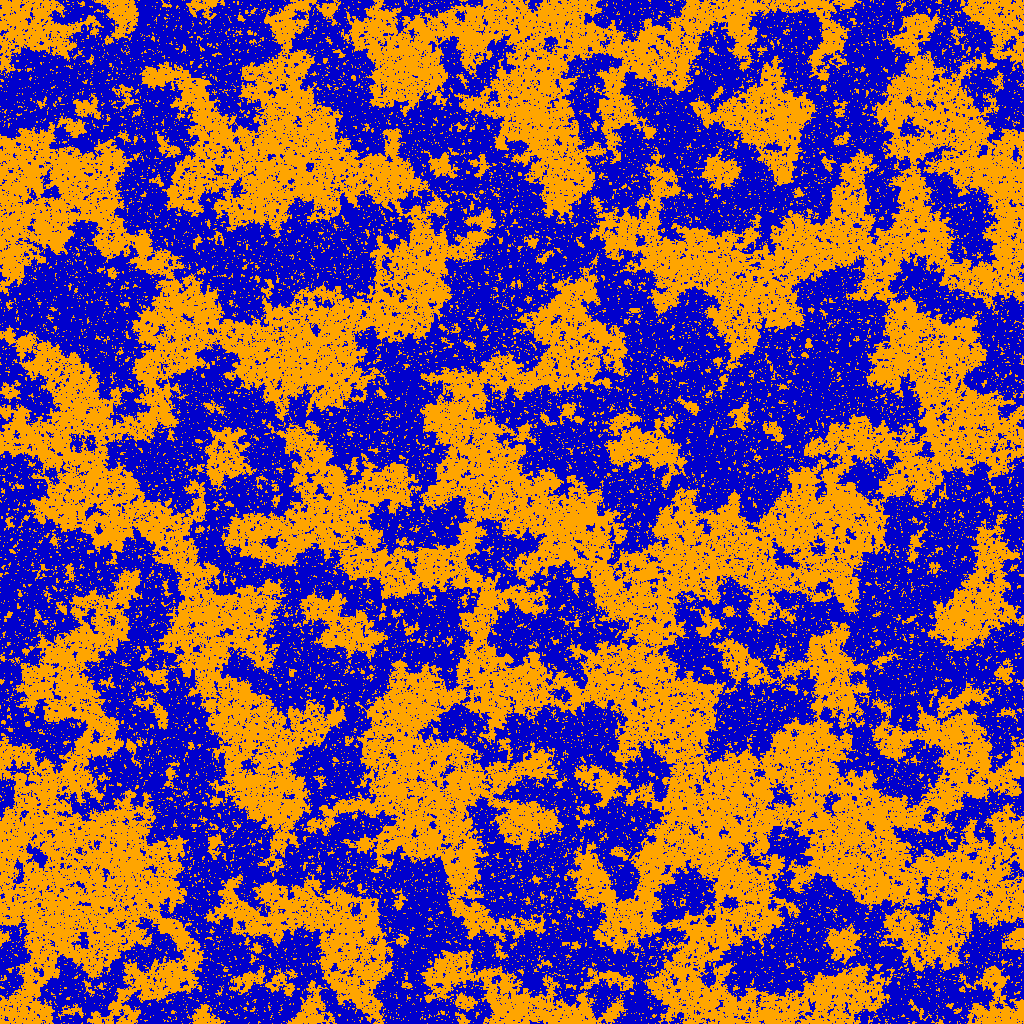
\includegraphics[width=\linewidth]{\fig/vis-0.45}
			\caption*{$J/(k_B T) = 0.45$}
		\end{subfigure}
		\begin{subfigure}{0.4\linewidth}
			\centering
			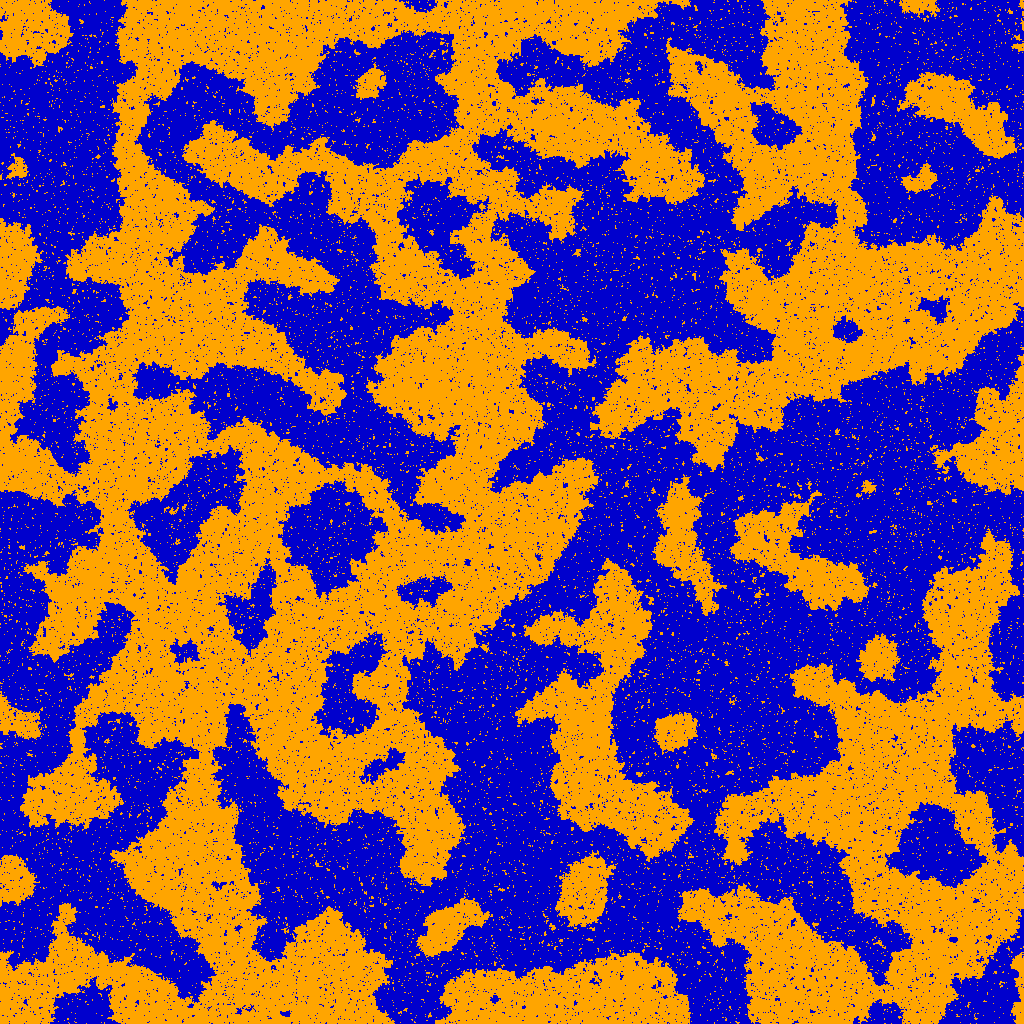
\includegraphics[width=\linewidth]{\fig/vis-0.5}
			\caption*{$J/(k_B T) = 0.5$}
		\end{subfigure}
		\begin{subfigure}{0.4\linewidth}
			\centering
			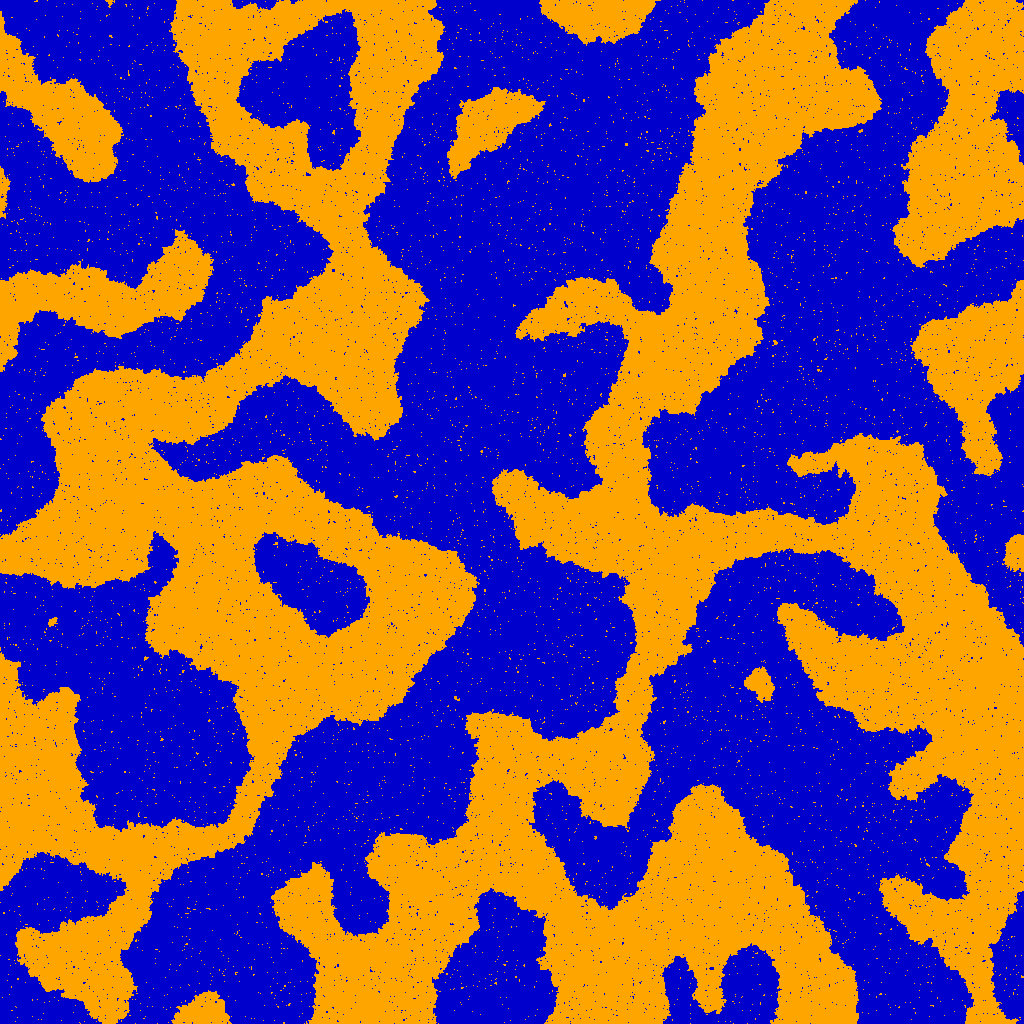
\includegraphics[width=\linewidth]{\fig/vis-0.6}
			\caption*{$J/(k_B T) = 0.6$}
		\end{subfigure}
	\end{figure}
\end{document}